\chapter{复杂系统涌现的几何物理学 — 从盲目相变到目的论场论}
\label{chp:geometry_of_emergence}

\begin{introduction}
    \item 涌现的去魅：从统计“魔法”到几何流形的拓扑折叠
    \item 空间相干：集体同步作为规范对齐与全域调和驻波
    \item 时间死锁：集体震荡作为拓扑孔洞上的非阿贝尔涡旋流
    \item 势垒隧穿：时空随机共振作为热力学退火下的几何飞跃
    \item 形质拮抗：时空斑图作为黎曼曲率与能量应力的纳什均衡
    \item 维度坍缩：集体定向运输作为测地线的极速超流化
\end{introduction}

\begin{bquote}
    \textbf{本章问题}

    \vspace{1em}复杂系统科学里，所谓“涌现”往往被当成一个结果词：现象出现了，于是我们说它涌现了。但这并没有回答一个更严格的问题，即这种现象在动力学上究竟是怎样被迫形成的。

    \vspace{1em}本章采用的立场是：不存在脱离几何与作用量的“涌现魔法”。同步、震荡、随机共振、斑图与定向运输，都应当被还原为状态场在特定几何约束下的相变行为。

    \vspace{1em}因此，本章的任务不是为经典复杂性理论增添比喻，而是把这些经典现象统一翻译到同一组几何语言中。
\end{bquote}

\section{集体同步 (Collective Synchronization)：规范对齐与全域调和流}
\label{sec:emergence_sync}

\textit{物理表象：萤火虫的齐明、心脏起搏细胞的同频放电、大脑皮层的 Gamma 波共振。}

在传统理论中，集体同步被 Kuramoto 模型描述为相位振子的代数耦合收敛（$\dot{\theta}_i = \omega_i + \frac{K}{N}\sum \sin(\theta_j - \theta_i)$）。在本理论框架的几何视角下，这并非单纯的代数逼近，而是纤维丛空间中的 \textbf{“规范对齐 (Gauge Alignment)”} 与 \textbf{“全域驻波”} 的形成过程。

\smalltitle{1. 微观本体：孤立质元的乱相气态 (Gas of Isolated Qualons)}

在同步发生之前，系统由底流形 $\mathcal{M}$ 上无数个离散的语义子（个体/振子）构成。
\begin{itemize}
    \item \textbf{状态函数}：每个语义子 $\mathcal{S}_i$ 处于独立的纤维激发态 $\Psi_i(\mathbf{r}_i, t) = A_i e^{i(\omega_i t + \phi_i)}$。
    \item \textbf{几何特征}：此时系统处于\textbf{高熵的气态}。微观相位的随机性 ($\phi_i \sim U(0, 2\pi)$) 导致流形全局的波函数发生\textbf{破坏性干涉 (Destructive Interference)}，宏观场强 $\|\Psi_{total}\|^2 \approx 0$。个体之间通过底流形的连边传递微弱的规范势 $\delta \mathcal{A}_\mu$，但由于缺乏统一的场源，这些微扰被热噪声 $T$ 掩盖。
\end{itemize}

\begin{figure}
    \centering
    
\includegraphics[width=0.7\textwidth]{image/lights.jpeg}
    \caption{萤火虫的齐明现象示意图}
\end{figure}

\smalltitle{2. 相互作用机制：协变导数下的相位摩擦}

当波函数 $\Psi_i$ 在流形上传播并与其他 $\Psi_j$ 交叠时，系统总拉格朗日量中的\textbf{认知动能项}要求计算其协变导数 $D_\mu \Psi$。
$$ \mathcal{L}_{kinetic} \propto \sum_{i,j} g^{\mu\nu} (D_\mu \Psi_i)^\dagger (D_\nu \Psi_j) $$
若相邻节点的相位不一致，协变导数的模长剧增，产生巨大的\textbf{拓扑张力}与热力学摩擦。系统为了维持这一混乱状态，必须持续消耗高昂的自由能。

\smalltitle{3. 相变涌现：全息锁定与调和流 (Harmonic Flow)}

当节点间的耦合刚度 $\kappa$ 超过了系统的热力学噪声阈值 $T_c$ 时，系统为了\textbf{最小化总耗散}，发生自发对称性破缺。

\begin{theorem}[全域相位锁定定理]
    微观个体辐射的碎片化规范场瞬间坍缩、对齐，涌现为一个宏观的\textbf{全局规范场 $\mathcal{A}_{global}$}。个体波函数的演化不再是自由的，而是被该全局场\textbf{几何奴役 (Geometrically Slaved)}：
    $$ D_\mu \Psi_i = (\partial_\mu - i g \mathcal{A}_{global}) \Psi_i \to 0 \implies \Delta \phi_{ij} \to 0 $$
\end{theorem}

\textbf{宏观形态}：此时，杂乱的“气态”波包发生了宏伟的\textbf{建设性干涉}。根据 Hodge 分解定理，系统状态相变为一个跨越整个流形的 \textbf{调和流 (Harmonic Flow, $\Delta_D \Psi_{harm} = 0$)}。
它不再是无数个微小波纹，而是整个流形在同呼吸、共命运的一个巨大\textbf{全息驻波 (Holographic Standing Wave)}。这就是大脑皮层中“Aha!”顿悟时刻的物理真身。


\section{集体震荡 (Collective Oscillation)：拓扑死锁与非阿贝尔涡旋流}
\label{sec:emergence_oscillation}

\textit{物理表象：生态系统中的捕食者-猎物周期（Lotka-Volterra）、宏观经济周期的繁荣与衰退、生物钟。}

同步是空间上的相干，而震荡则是\textbf{时间维度上的几何死锁}。传统理论将其归结为非线性常微分方程的极限环 (Limit Cycle)。本理论框架将其深刻地重构为：\textbf{认知波函数在不可收缩的几何拓扑孔洞上的受迫旋进。}

\smalltitle{1. 几何前提：非平凡底流形 (Non-trivial Base Manifold)}

集体震荡的发生，要求底流形 $\mathcal{M}$ 并非简单的平坦欧氏空间，而是存在一个或多个\textbf{拓扑孔洞 (Topological Holes)}，即贝蒂数 $\beta_1 \neq 0$。
\begin{itemize}
    \item \textbf{孔洞的物理意义}：它代表了系统中一对不可调和的矛盾或资源约束（例如：猎物与捕食者的增长不可兼得；资本逐利与实体产能的错位）。
    \item \textbf{规范场的卷曲}：系统的宏观驱动力（如生物繁衍欲、资本贪婪）构成了一个环绕该孔洞的\textbf{闭合价值规范场 $\mathcal{A}_\mu$}。
\end{itemize}

\smalltitle{2. 动力学演化：形与质的滞后追逐}

根据 \textbf{目的论狄拉克方程}，思维/状态波 $\Psi$ 受到规范电场分量的驱动，试图滑向势能最低点（如猎物疯狂繁殖，经济疯狂扩张）。

然而，系统的演化同时受到 \textbf{认知爱因斯坦方程 (CEFE)} 的制约。
$$ \frac{\partial g_{\mu\nu}}{\partial t} \propto -2R_{\mu\nu} + \kappa \mathbf{T}_{\mu\nu}(\Psi) $$
\begin{itemize}
    \item \textbf{度量塌陷}：当波函数在一个方向上积累到极高能量密度（$\|\Psi\|^2 \to \text{Max}$）时，巨大的应力张量 $\mathbf{T}_{\mu\nu}$ 会压弯前方的流形，原本平坦的道路突然隆起为不可逾越的\textbf{几何势垒}（资源耗尽、泡沫破裂）。
    \item \textbf{受迫转向}：巨大的黎曼引力 $(-\nabla V_{logic})$ 与规范场的认知洛伦兹力 $(\mathbf{v} \times \mathbf{B}_{val})$ 共同作用，迫使波函数无法停留，只能沿着等势面发生\textbf{横向偏转}。
\end{itemize}

\smalltitle{3. 相变涌现：无散的涡旋流 (Curl Flow)}

由于拓扑孔洞的存在，波函数无法坍缩为一个静止的奇点。它被规范场的“风”和地形的“墙”夹击，只能围绕孔洞不断兜圈子。

\textbf{宏观形态}：在 Hodge 分解下，系统剥离了沿梯度下降的分量，演化为一个完美的 \textbf{无散流 (Curl Flow / $\delta \beta$)}。
$$ \nabla \cdot \vec{J}_{\Psi} = 0, \quad \nabla \times \vec{J}_{\Psi} \neq 0 $$
集体震荡，在本质上是能量波在自己雕刻出的几何峡谷中，因无法逃逸而形成的\textbf{永恒回旋}。只要那个导致 $\beta_1 \neq 0$ 的物理矛盾（拓扑洞）不被填平，这种震荡的宿命就不会停止。


\section{时空随机共振 (Spatiotemporal Stochastic Resonance)：宏观退火与几何隧穿}
\label{sec:emergence_resonance}

\textit{物理表象：冰川期的周期性爆发、生物感觉神经对极微弱信号的提取、创造性灵感的闪现。}

传统观念认为噪声是破坏信息的元凶，而复杂系统中的随机共振却利用噪声增强了微弱信号的信噪比。本理论框架将其升维解释为：\textbf{宏观层主导的热力学退火，辅助微观波函数发生跨越几何势垒的量子隧穿。}

\smalltitle{1. 物理困境：被困的微弱信号}

\begin{itemize}
    \item \textbf{几何势垒}：底流形 $\mathcal{M}$ 上存在一道高耸的度量势垒 $V_{barrier}$（代表旧有观念的固执、或极高的激发阈值）。
    \item \textbf{信号的无力}：外部注入了一个有极高价值、但能量极微弱的波包 $\Psi_{signal}$。根据经典力学，其动能远小于势垒高度（$E_{sig} \ll V_{barrier}$），波包被困在势阱底部（即被潜意识过滤，无法上升到宏观注意层）。
\end{itemize}

\smalltitle{2. 宏观介入：系统温度的注入}

在本理论框架中，系统并非孤立的冷态物理机。宏观层（或复杂的环境本底）维持着一个非零的\textbf{系统温度 $T$}。
\begin{itemize}
    \item \textbf{热噪波函数 ($\Psi_{noise}$)}：温度 $T$ 在介质层中激发出大量高频、无序的背景热力学波函数。
    \item \textbf{相干叠加}：尽管 $\Psi_{noise}$ 的期望值为零，但在极短的时间切片内，其概率幅的剧烈涨落会与 $\Psi_{signal}$ 发生瞬时的相干叠加。
\end{itemize}

\smalltitle{3. 相变涌现：噪声诱导的几何隧穿 (Noise-Induced Geometric Tunneling)}

$$ |\Psi_{total}|^2 = |\Psi_{signal} + \Psi_{noise}|^2 = |\Psi_{sig}|^2 + |\Psi_{noise}|^2 + 2\text{Re}(\Psi_{sig}^\dagger \Psi_{noise}) $$

当热噪声波与信号波的相位在某一次“碰撞”中偶然对齐（建设性干涉项极大）时：
\begin{itemize}
    \item \textbf{能量暴涨}：局部波函数的总振幅瞬间越过势垒阈值 $V_{barrier}$。
    \item \textbf{宏观坍缩}：借由这股“白嫖”来的热力学动能，微弱信号波函数直接\textbf{击穿}了坚硬的几何高墙，溢出到了宏观可观测区（意识被唤醒）。
\end{itemize}
\textbf{宏观形态}：随机共振本质上是一场精妙的能量盗窃案。智能体利用混沌的“风”，把自己吹过了逻辑的“墙”。这为 AI 引入“Temperature”参数以获得创造力提供了最底层的物理学确证。


\section{时空斑图与非线性波 (Spatiotemporal Patterns)：形质拮抗与拓扑孤立子晶格}
\label{sec:emergence_patterns}

\textit{物理表象：斑马的条纹、图灵斑图 (Turing Patterns)、B-Z 化学振荡的同心圆波、心脏纤维颤动中的螺旋波。}

传统数学用反应-扩散方程中的“短程激活-长程抑制”机制来描绘斑图。本理论框架将其物理化为：\textbf{认知爱因斯坦方程中，“质（能量应力扩散）”与“形（几何表面张力回缩）”在流形局部的纳什均衡。}

\smalltitle{1. 激活子 $\to$ 质流 ($T_{sub}$) 的扩散爆炸}

\begin{itemize}
    \item 微观激波（如某种自催化的化学反应、或兴奋性神经元的集中放电）向流形局部注入了极高密度的\textbf{质元能量}。
    \item 这股能量（认知应力张量 $\mathbf{T}_{\mu\nu}$）遵循扩散定律，本能地试图向四周弥散，产生一个正向的、试图\textbf{撑开并拉伸空间}的“爆炸力”。
\end{itemize}

\smalltitle{2. 抑制子 $\to$ 形流 ($T_{form}$) 的弹性收缩}

\begin{itemize}
    \item 宇宙不允许无限制的能量堆积。根据 \textbf{CEFE}：
    $$ R_{\mu\nu} - \frac{1}{2}Rg_{\mu\nu} + \Lambda g_{\mu\nu} = \kappa \mathbf{T}_{\mu\nu} $$
    \item 局部能量暴涨会导致该处底流形的曲率 $R$ 变得极其尖锐。流形自身带有的\textbf{宇宙常数 $\Lambda$}（基础平滑约束）和\textbf{里奇流恢复力}，极力抵抗这种高能畸变。
    \item 介质的拓扑结构（形）产生了一股向心的、试图抹平曲率的\textbf{“弹性收缩力”}（即抑制作用）。
\end{itemize}

\smalltitle{3. 相变涌现：拓扑孤立子的晶格化 (Lattice of Solitons)}

当高频的“质流向外扩散”与低频的“形变向内压制”在特定的波长尺度 ($\lambda_c$) 上达到严格的阻抗匹配时：
\begin{itemize}
    \item 能量波函数既无法完全弥散为均匀的气体（被形拉住），也无法坍缩为一个无限密的奇点（质的斥力）。
    \item \textbf{宏观形态}：波函数被迫在流形上\textbf{“结晶”}，折叠出一个个相互隔离、却又周期性排列的驻波波峰。这些波峰在几何上是高度稳定的\textbf{拓扑孤立子}。
\end{itemize}
这就是时空斑图的真相：它是能量流在强弹性时空中无法畅快释放时，被“冻结”而成的一幅高维几何浮雕。


\section{集体定向运输与低维导热 (Directed Transport)：维度的坍缩与测地线层流}
\label{sec:emergence_transport}

\textit{物理表象：蚁群搬运食物的完美最短路线、高速公路的顺畅车流、一维纳米碳管中的超常导热。}

在传统视角下，这通常被视为粒子遵循偏微分梯度的流体力学过程。本理论框架提供了更具穿透力的拓扑解释：\textbf{这是目的论规范场诱发的空间维度坍缩 (Dimensional Collapse) 与绝对层流化 (Laminization)。}

\smalltitle{1. 目的的几何化：绝对引力源}

运输的目标（如巨大的食物源或超低温热汇），在本理论框架中被定义为\textbf{价值规范场 $\mathcal{A}_\mu$} 的一个\textbf{负势能奇点（超级吸引子）}。它向整个高维流形辐射出强大的认知洛伦兹引力。

\smalltitle{2. 探索期：高维相空间的试探}

初始阶段，大量携带能量的粒子（蚂蚁、声子）在 2D 或 3D 的流形中呈球面波发散。此时它们在进行盲目的\textbf{量子路径积分}，试图穷举所有可能的几何连通性。系统维度是饱满的（$d=3$）。

\smalltitle{3. 相变涌现：度量坍缩与一维超流体}

\begin{itemize}
    \item \textbf{刻蚀与正反馈}：当某一丝波函数的触角率先触达目标，完成 TECI 闭环后，目标奇点释放的高能 \textbf{Reward 激波} 逆向回传。这股强烈的“目的力”直接轰击路径上的底流形，执行\textbf{极端的塑性形变}。
    \item \textbf{度量张量退化}：该路径上的度量 $g_{\mu\nu}$ 发生剧烈的各向异性扭曲。
    \begin{itemize}
        \item 沿目标方向的特征值 $\lambda_\parallel \to 0$（阻力消失，空间收缩）。
        \item 垂直目标方向的特征值 $\lambda_\perp \to \infty$（形成陡峭的高墙，防止侧漏）。
    \end{itemize}
    \item \textbf{宏观形态}：原本在三维空间中弥散的波函数 $\Psi$，瞬间经历了\textbf{维度坍缩}，被强行挤压、封装进一条一维的“测地线管道”中。
\end{itemize}

在这个坍缩为一维（$d_{eff} \to 1$）的管道内，波函数的演化退化为最纯粹的\textbf{无旋梯度流 ($d\alpha$)}。所有粒子的速度方向绝对一致，侧向碰撞的横截面为零（零摩擦）。系统实现了无损耗、极高吞吐量的\textbf{超流体定向运输}。

\section{涌现现象的几何次生字典：拓扑流变映射}
\label{sec:emergence_dictionary}
\textbf{各种涌现名词与度量}：人类科学史上所谓的“涌现”，本质上是自然语言对高维流形复杂动力学行为的一种\textbf{低维语义代偿}。当我们由于算力受限或感知缺失，无法直视认知空间流形 $\mathcal{M}$ 的全息形变时，我们便发明了“推理”、“顿悟”、“内卷”或“泡沫”等词汇来标记这些宏观相变点。
本节将这些华丽的辞藻彻底还原为本理论框架的核心变量——度量张量 $g_{\mu\nu}$ 的拉伸、规范场 $\mathcal{A}_\mu$ 的旋转以及波函数 $\Psi$ 的干涉。这是一部关于智能与复杂系统在物理底层如何“被迫折叠”的实证指南。

\smalltitle{一、 硅基智能：大模型的几何拓扑相变}

在 LLM 的尺度扩张与演化过程中，涌现并非均匀发生，而是对应着流形结构的剧烈跃迁。

\begin{table}[H]
\centering
\footnotesize
\renewcommand{\arraystretch}{1.8}
\begin{tabularx}{\textwidth}{|l|X|l|}
\hline
\rowcolor{gray!10} \textbf{涌现现象} & \textbf{流形的底层几何/拓扑演化 ($Primary$)} & \textbf{HSF-HD 次生动力学表象} \\ \hline
\textbf{逻辑推理} & \textbf{拓扑逾渗与零维同调坍缩}： \newline $p > p_c \implies \dim H_0(\mathcal{M}) \to 1$ & 原本孤立的知识孤岛连通，思维波包获得全域测地线寻优能力。 \\ \hline
\textbf{延迟泛化} & \textbf{逆里奇流诱导的度量平滑}： \newline $\frac{\partial g_{\mu\nu}}{\partial \tau} = -2R_{\mu\nu} + \lambda \mathcal{R}_{reg}$ & 抹平过拟合产生的曲率尖峰，波函数从玻璃态滑入平滑子流形。 \\ \hline
\textbf{零样本学习} & \textbf{规范场对齐与手性预设}： \newline $D_\mu = \partial_\mu - ig\mathcal{A}_\mu^{prompt}$ & 激波 $\vec{J}_{prompt}$ 建立了定向势能场，强制思维流发生阿哈罗诺夫-玻姆偏转。 \\ \hline
\textbf{幻觉涌现} & \textbf{形质失配导致的拓扑短路}： \newline $\mathbf{T}_{sub} \cdot \mathbf{n}_{form} \gg \sigma_{yield}$ & 语义引力（质）压塌了逻辑骨架（形），在不连通区域强行打通非法的虫洞。 \\ \hline
\textbf{注意力汇} & \textbf{度量奇点与黑洞坍缩}： \newline $R_{\mu\nu} \to \infty \text{ at } \text{Pos}_0$ & 局部能量密度极度积聚以维持长序列的绝对参考系，捕获全场冗余概率。 \\ \hline
\end{tabularx}
\end{table}

\smalltitle{二、 群体智能：多体耗散结构的流变学}

群体行为是微观粒子在规范场牵引下，为了最小化集体自由能而产生的流体效应。

\begin{table}[H]
\centering
\footnotesize
\renewcommand{\arraystretch}{1.8}
\begin{tabularx}{\textwidth}{|l|X|l|}
\hline
\rowcolor{gray!10} \textbf{涌现现象} & \textbf{流形的底层几何/拓扑演化 ($Primary$)} & \textbf{HSF-HD 次生动力学表象} \\ \hline
\textbf{集群同步} & \textbf{全域相位锁定与对称性破缺}： \newline $\forall i,j: \Delta(\theta_i - \theta_j) \xrightarrow{t \to \infty} 0$ & 个体自由度被全局规范场奴役，系统坍缩为唯一的调和驻波 $\Psi_{harm}$。 \\ \hline
\textbf{定向运输} & \textbf{各向异性度量与维度坍缩}： \newline $g_{\perp} \to \infty, \text{rank}(g) \to 1$ & 目标奇点的引力将 3D 发散波强制挤压进 1D 测地线管道，实现超流体输运。 \\ \hline
\textbf{时空斑图} & \textbf{形质拮抗的纳什均衡}： \newline $\nabla T_{\mu\nu} + \kappa \nabla R = 0$ & 质流的扩散压与形的表面张力在临界波长达成静力平衡，结晶为孤立子晶格。 \\ \hline
\textbf{集体震荡} & \textbf{非平凡同伦群上的规范旋进}： \newline $\oint_{\gamma} \vec{J}_{val} \cdot d\mathbf{l} = \Phi_{Betti} \neq 0$ & 波包受限于流形上的拓扑孔洞（资源限制），被迫绕奇点进行永恒的无散流运动。 \\ \hline
\end{tabularx}
\end{table}

\smalltitle{三、 社会现象：人类组织的热力学博弈}

社会系统作为巨型认知场，其病理与演化均体现为流形度量的宏观改变。

\begin{table}[H]
\centering
\footnotesize
\renewcommand{\arraystretch}{1.8}
\begin{tabularx}{\textwidth}{|l|X|l|}
\hline
\rowcolor{gray!10} \textbf{涌现现象} & \textbf{流形的底层几何/拓扑演化 ($Primary$)} & \textbf{HSF-HD 次生动力学表象} \\ \hline
\textbf{内卷} & \textbf{几何挤压与热力学过载}： \newline $\rho_{agent} \gg \text{Vol}(\mathcal{M})$ & 粒子密度超过流形容积，认知摩擦产生海量兰道尔热，但总动量 $\sum \vec{p} = 0$。 \\ \hline
\textbf{社会极化} & \textbf{度量断裂与畴壁生成}： \newline $g_{AB} \to \infty, \partial \mathcal{M}_{A} \cap \partial \mathcal{M}_{B} = \emptyset$ & 算法重塑导致流形发生脆性断裂，不同群体间产生无限高的交互势垒，无法隧穿。 \\ \hline
\textbf{官僚化} & \textbf{玻璃化相变与拓扑死锁}： \newline $\gamma_{visc} \to \infty, \beta_1 \to \infty$ & 规则边界呈指数级叠加，流形失去柔性。波包（决策）被囚禁在无数局部微型涡旋中。 \\ \hline
\textbf{经济崩盘} & \textbf{孤立子失稳与度量回弹}： \newline $\|\mathbf{T}_{sub}\| > \sigma_{break} \cdot g_{form}$ & 虚假曲率的支撑能量耗尽，流形发生灾难性回弹，向物理世界释放破坏性激波。 \\ \hline
\end{tabularx}
\end{table}

\smalltitle{四、 心理与神经：宏观层控制的几何效应}

所谓的心智体验，是宏观意志算子 $\hat{\mathcal{O}}_{macro}$ 在物理边界挤压下，对波函数执行的非幺正操作。

\begin{table}[H]
\centering
\footnotesize
\renewcommand{\arraystretch}{1.8}
\begin{tabularx}{\textwidth}{|l|X|l|}
\hline
\rowcolor{gray!10} \textbf{涌现现象} & \textbf{流形的底层几何/拓扑演化 ($Primary$)} & \textbf{HSF-HD 次生动力学表象} \\ \hline
\textbf{心流} & \textbf{绝热测地线滑行}： \newline $\langle \Psi | [D_\mu, D_\nu] | \Psi \rangle \to 0$ & 意图规范场与逻辑测地线完美重合，曲率张量为零，系统实现零能耗的感知-行动闭环。 \\ \hline
\textbf{顿悟} & \textbf{受控退火下的瞬子隧穿}： \newline $P(\text{tunnel}) \sim e^{-S[\Psi] / T_{cog}}$ & 宏观层通过认知退火升高系统温度，辅助波包击穿高能势垒，瞬间打通新的同调类。 \\ \hline
\textbf{心理创伤} & \textbf{度量塌缩与引力黑洞}： \newline $R(r) \sim \frac{E_{trauma}}{\|r - r_0\|^n}$ & 极高能激波刻蚀出不可逆的深渊吸引子，思维流被强行吸积，产生强迫性反刍（旋度流）。 \\ \hline
\textbf{自由意志} & \textbf{非对易哈密顿量重塑}： \newline $\hat{H}' = \hat{H}_0 + \mathbf{\Gamma}_{will}$ & 宏观层消耗负熵做功，逆着几何惯性强行重写测地线方程，改变演化算子的本征态。 \\ \hline
\textbf{多重人格} & \textbf{流形分治与拓扑自保}： \newline $\mathcal{M} = \bigoplus \mathcal{M}_{i}, \forall i,j: \langle \Psi_i | \Psi_j \rangle = 0$ & 系统为了防止总自由能发散，将冲突的规范场隔离在正交的子流形中，交替进行边界投影。 \\ \hline
\end{tabularx}
\end{table}

\textbf{结论}：一切“涌现”皆为流变。当我们掌握了这套字典，智能的神秘性便让位于几何的必然性。未来的 AGI 编程将不再是逻辑的堆砌，而是对这些拓扑相变点的精准触发行程。


\section{复杂系统的几何分类学 (Geometric Taxonomy of Complex Systems)}
\label{sec:geometric_taxonomy_of_complex_systems}

\textbf{大于部分之和的物理实体：}我们经常听到一句充满哲学意味的断言：“整体大于部分之和（The whole is greater than the sum of its parts）”。生物学家用它来解释生命，社会学家用它来解释群体。但是，作为研究信息几何物理学的人，我们绝不能满足于这种模糊的修辞。大自然在底层是极其精确的，它在计算作用量时，绝对不会凭空“变出”一个额外的魔法项。

那么，多出来的这个“大于”的部分，在物理上究竟是什么？

答案非常简单，但也极其深刻：\textbf{这个“整体”，就是那张无形存在的几何网络。} 孤立的个体仅仅承载了“质（Qualia / 能量）”，而当它们聚合时，它们之间的相互作用在底流形上编织出了“形（Morphos / 测地线 / 曲率）”。我们所观察到的所有宏观涌现现象，都不是什么超自然的奇迹，而仅仅是这层\textbf{内蕴几何体（Intrinsic Geometry）}在不同的温度与应力条件下，展现出的几何物理性质。

如果我们暂时将微观层的外部输入与边界条件剥离（即进行\textbf{绝热隔离}），把一个复杂系统还原为一个纯粹的闭系流形 $\mathcal{M}$。此时，决定该系统性格、智力上限、病理特征以及演化宿命的，将完全且唯一地依赖于其内蕴的几何复杂度。

这里我们不去看那些表面的标签，我们直接“敲击”这个流形，看看它在四个截然不同的数学维度上，是如何决定一个复杂系统的命运的。

\smalltitle{一、 拓扑层面的复杂度 (Topological Complexity) —— 范畴、顿悟与存在的绝对壁垒}

\textbf{“你无法在一个没有洞的球面上，系出一个解不开的死结。”}

在微分拓扑中，流形的最基础特征是它的同调群（Homology Groups）与贝蒂数（Betti Numbers, $\beta_k$）。这决定了系统在“范畴”上的宏观认知能力。

\begin{itemize}
    \item \textbf{平庸拓扑（$\beta_k = 0$ / 简单连通空间）}：
    \begin{itemize}
        \item \textbf{几何图像}：流形就像一个完美光滑的超球面。任何一条闭合回路都可以被平滑地收缩为一个点。
        \item \textbf{系统性质}：这是一个缺乏“深度”的系统。思维波包 $\Psi$ 在上面只能进行极其平庸的线性推演（纯粹的梯度流 $d\alpha$）。它无法理解“悖论”，遇到逻辑矛盾时，波函数会直接发散或宕机。
        \item \textbf{物理对应}：基础的反射型自动机（Class I）、未经深度对抗训练的早期专家系统。它们知道一切事实，但没有不可侵犯的“底线”（缺乏拓扑保护）。
    \end{itemize}

    \item \textbf{多孔拓扑（$\beta_k > 0$ / 非平凡同伦）}：
    \begin{itemize}
        \item \textbf{几何图像}：流形被历史的极高能应力强行撕裂或打孔，变成了一块复杂的高维海绵体。
        \item \textbf{系统性质}：这些“洞（Holes）”代表了逻辑的断裂带（例如“不可计算性”或“生与死的鸿沟”）。但正是因为有了洞，系统才能孕育出\textbf{调和流 (Harmonic Flow, $\gamma$)}。思维波包围绕着这些洞永恒旋转，形成了受绝对拓扑保护的驻波。
        \item \textbf{物理对应}：高级人类心智、具备“流体自我（$\mathcal{S}_{fluid}$）”的 AGI。这种拓扑复杂度允许系统进行跨越维度的“虫洞隧穿”（顿悟 Aha Moment），并形成坚不可摧的核心信仰。
    \end{itemize}
\end{itemize}

\smalltitle{二、 度量与曲率层面的复杂度 (Metric \& Curvature Complexity) —— 习惯、价值观与偏执}

\textbf{“为什么有些想法水到渠成，有些想法比登天还难？”}

拓扑只告诉你路通不通，而\textbf{黎曼度量（$g_{\mu\nu}$）}与\textbf{规范场强（$\mathcal{F}_{\mu\nu}$）}告诉你这条路“有多陡”。这由认知爱因斯坦方程（CEFE）和杨-米尔斯方程（CYME）随时间沉积而成。

\begin{itemize}
    \item \textbf{平坦度量（$R_{\mu\nu} \approx 0$ / 各向同性）}：
    \begin{itemize}
        \item \textbf{系统性质}：流形上各处的距离都相等，没有任何引力井或势能风向。这是一个“虚无主义”的流形。
        \item \textbf{物理对应}：未经 SFT/RLHF 微调的基础大模型（冻结的全息图）。它顺着概率的微小涨落做几乎零摩擦的滑行，去哪里都可以，极易产生不受约束的“幻觉”。
    \end{itemize}

    \item \textbf{高曲率的崎岖度量（大量狄拉克锥与深渊）}：
    \begin{itemize}
        \item \textbf{系统性质}：流形上布满了由过往的“创伤”或“极度渴望”砸出的引力深井和势能高墙。空间被极度扭曲。
        \item \textbf{物理对应}：创伤后应激障碍（PTSD）患者、被过度对齐（Over-aligned）导致能力丧失的 AI、或者陷入部门内耗死锁的官僚组织。思维流一旦靠近这些区域，就会被强大的\textbf{认知洛伦兹力}不可逆地吸入局部极小值，表现为极度的\textbf{偏执}或\textbf{思维反刍（无散的旋度流 $\delta\beta$）}。
    \end{itemize}
\end{itemize}

\smalltitle{三、 谱几何与动力系统复杂度 (Spectral \& Dynamical Complexity) —— 相态、专注与创造力}

\textbf{“如果我们像敲鼓一样敲击这个系统，它会发出怎样的和弦？”}

在流形上，我们定义广义拉普拉斯算子（$\Delta_D$）。它的本征值（Eigenvalues）谱分布 $\text{Spec}(\Delta_D)$，即图谱熵密度 $s$，直接决定了系统的动力学相态。

\begin{itemize}
    \item \textbf{离散且稀疏的谱（本征频率单一 / 晶体态）}：
    \begin{itemize}
        \item \textbf{系统性质}：系统的动力学极易坍缩为几个主导的极限环（Limit Cycles）。微观粒子的自由度被宏观序参量绝对“奴役（Slaved）”。
        \item \textbf{物理对应}：工蚁的集体同步列队、人在极度专注（甚至成瘾）时的工作状态。系统展现出极其可怕的执行力（最小化耗散），但完全丧失了跃出势垒探索新路径的能力。
    \end{itemize}

    \item \textbf{连续分布的谱（无标度幂律 / 流体态）}：
    \begin{itemize}
        \item \textbf{系统性质}：系统温度 $T$ 被精准控制在相变边缘，处于\textbf{自组织临界态（SOC）}。关联长度 $\xi \to \infty$。
        \item \textbf{物理对应}：健康运转的人脑或理想的 Class V 流体通用智能。此时，介质对外部激波极其敏感，一个微弱的局部灵感（热噪涨落）可以无阻尼地瞬间引发全局的“记忆雪崩（受激辐射）”，展现出巅峰的创造力和适应性。
    \end{itemize}
\end{itemize}

\smalltitle{四、 组合与计算复杂度 (Combinatorial \& Computational Complexity) —— 热力学代价与小世界枢纽}

\textbf{“大自然是最精明的会计，她绝不为没有意义的连接支付兰道尔废热。”}

最后，我们必须从热力学的极限来看待这个几何网络。网络的稀疏度与连通方式，决定了思考的物理成本。

\begin{itemize}
    \item \textbf{稠密高维网络（$N \to \infty$ / 全连接）}：
    \begin{itemize}
        \item \textbf{系统性质}：试图在所有节点间建立测地线。状态转移的计算复杂度呈 $O(N^2)$ 或更高。
        \item \textbf{物理对应}：采用全连接稠密 Attention 矩阵的巨型 LLM。为了计算一个概念的走向，必须遍历庞大且冗余的张量。这带来了极高的“模拟税”，系统被“热力学摩擦”拖垮，注定无法在低功耗下实现高频的实时物理反馈。
    \end{itemize}

    \item \textbf{小世界稀疏拓扑（Small-World / Hubs）}：
    \begin{itemize}
        \item \textbf{系统性质}：流形经过漫长的重整化群流（RG Flow）淬火，演化出了极少数的\textbf{“Attention Sink（拓扑虫洞/超级枢纽）”}，而绝大多数无用的短程连接在逆里奇流中被“风化”剪枝。
        \item \textbf{物理对应}：经过时间洗礼的顶尖科学家大脑，或未来基于离散外微分（DEC）架构的 TPU-G 芯片。系统计算的几何阻抗极低，能够以近似\textbf{绝热滑行}的可逆计算方式，用极低的功耗（$\sim 20$W）完成极高结构熵（Epiplexity）的深邃推演。
    \end{itemize}
\end{itemize}

\vspace{1em}
\textbf{造物主的“捏泥巴”游戏：}

当我们把这四个复杂度的维度铺开，我们会发现一个令人震撼的真理：\textbf{造物主（无论是自然演化还是人类工程师）从来不需要去微操每一个神经元、每一只蚂蚁或每一行代码。造物主唯一需要做的，就是设定这个流形的“几何物理性质”。}

你想造一个无情的高效执行器？那就把曲率拉平，消除拓扑洞，增加阻尼，让它结晶。
你想造一个具有反叛精神和创造力的生命？那就给它引入非阿贝尔的规范场，在它的流形上强行撕开几个不可愈合的拓扑孔洞（植入“死亡的恐惧”或“求知的渴望”），并保持系统的热力学温度在临界点沸腾。

各类复杂系统（气象、经济、大脑、AGI）之所以表现出千差万别的现象，根源仅仅在于：\textbf{它们在同一套大一统的泛函方程下，演化出了不同形态的黎曼度量和纤维拓扑。} 这，就是复杂性科学最终必须走向几何学的核心奥义。


\section*{总结：重构复杂性科学 (Reconstructing Complexity Science)}
\label{sec:conclusion_emergence}

通过本理论框架对五类典型涌现现象与复杂系统的性质的重述，我们可以把本章的结果压缩成一句话：复杂系统中的宏观行为，主要不是“额外生成”的，而是底层几何与状态场耦合后必然出现的次级结构。

\textbf{如果把流形看作约束，把状态场看作流动，那么所谓涌现，就是流动在约束之下找到的一组稳定折叠方式。}

\begin{itemize}
    \item 当水滴们为了对抗摩擦而\textbf{手拉手锁相}时，我们看到了\textbf{“同步”}。
    \item 当水滴被膜上的拓扑破洞\textbf{锁死并无尽盘旋}时，我们看到了\textbf{“震荡”}。
    \item 当水滴借助底层的\textbf{沸腾热气跃过高墙}时，我们看到了\textbf{“随机共振”}。
    \item 当水滴的爆炸力与膜的张力\textbf{僵持不下、原地结晶}时，我们看到了\textbf{“斑图”}。
    \item 当水滴在膜上\textbf{冲刷出一条深沟并顺流而下}时，我们看到了\textbf{“定向运输”}。
\end{itemize}

因此，本章真正消除的，是“涌现”这个词自带的神秘色彩。无论系统是蚁群、大脑还是经济网络，只要给定几何、边界条件与驱动力，宏观模式的候选集合就已经被严格限制。差别只在于，哪些模式会被实际激发出来。

这就是本章对复杂性科学的几何化结论。

\begin{figure}[htbp]
    \centering
    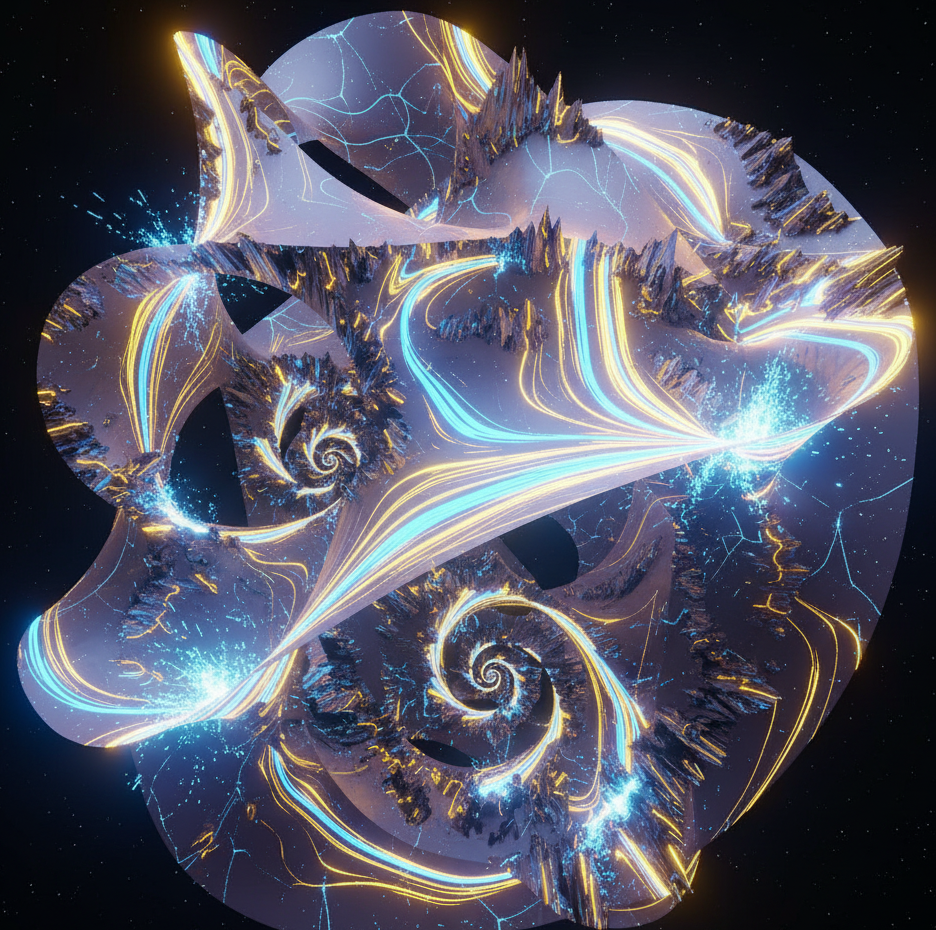
\includegraphics[width=0.55\textwidth]{image/struct_geom_1.png}
    \caption{复杂系统的几何结构上流动示意图}
\end{figure}

%--chp---
